\documentclass[11pt,lineno]{../_configs}

\articletype{Theoretical} % article type

\bibliography{SFC.bib}

\newcommand{\getkey}{caiani_agent_2016}

\newcommand{\autor}{\textcite{\getkey} }

\title{
\large{SFC}\vspace{2pt}\\
\Huge{\autor - \citetitle*{\getkey}}
}
\date{April 22th, 2020}

\author[$\ast$]{Gabriel Petrini}

\affil[$\ast$]{PhD Student at Unicamp.}

\keywords{
	Agent Based Macroeconomics\\
	Stock Flow Consistent Models\\
	Business Cycles\\
	Bank Regulation
	
}

\runningtitle{Sillabus} % For use in the footer 

%% For the footnote.
\runningauthor{Petrini}

\begin{abstract}
\abssection{Background} Great Recession imposed some challenges to standard orthodox macroeconomic models (notably DSGE) in which --- besides its improvements --- there are still drawbacks: money endogeneity, complexity and fallacy of composition. Authors argue that DSGE models depends on external shocks in order to explain the origins of non-linearities.

\abssection{Supporting ideas} 

\abssection{Contribution} Proposes a set or rules and tools to build, calibrate, validate, and display AB-SFC models.

\abssection{Relevance} Brings some ideas to introduce AB-SFC in FAPESP project. Presents some advantages in using SFC models, such as: (i) logical consistency check; (ii) adequacy in modeling endogenous and government money. The authors also maps some critics such as highly aggregate models and does not allow to analyze agents’ heterogeneity and agents’ disperse interaction. This critic is overcome by AB a proposal in which economy is seen as a complex adaptive system.

\abssection{Methods} A fully decentralized AB-SFC model. \textbf{Validation:} numerical simulations are compared to some micro and macro stylized facts. \textbf{Calibration:} Employ sensitivity experiments

\abssection{Results} Simulations reports some empirical regularities

\abssection{Interesting findings} 

\abssection{Critics} 
 \end{abstract}

\begin{document}

\maketitle
\articletypemark
\marginmark
\thispagestyle{firststyle}
% Please add here a significance statement to explain the relevance of your work

\noindent \textbf{Citation:} 	\fullcite{\getkey}

\begin{infobox}
	\textbf{5SS:} \autor 
\end{infobox}


\begin{figure}
	\centering
	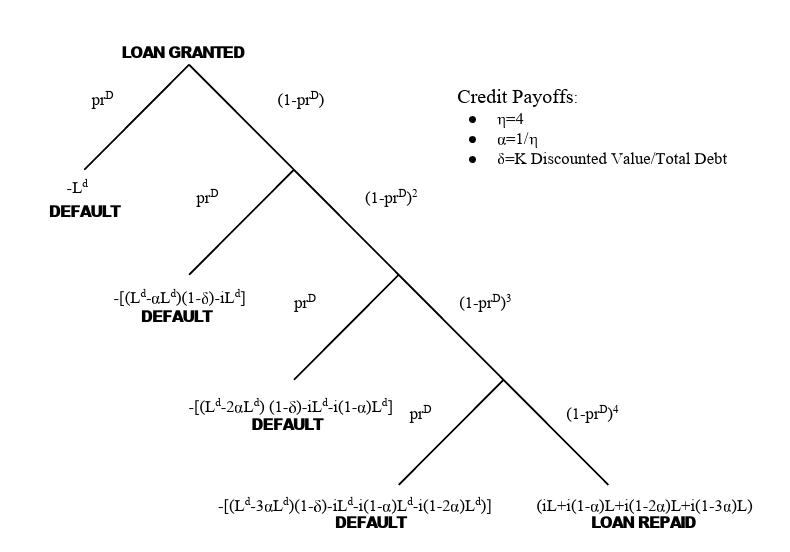
\includegraphics[width=0.7\linewidth]{figs/caiani_agent_2016_001}
	\caption{}
	\label{fig:caianiagent2016001}
\end{figure}


\begin{redbox}{Further readings}
	\begin{description}
		\item[Farmer and Foley (2009):] ABM approach
		\item[Esptein (2006):] ABM approach 
		\item[Delli Gatti et al., (2010a)]: Fallacy composition in DSGE models
	\end{description}
\end{redbox}

\printbibliography
	
\end{document}
